


\tikzset{every picture/.style={line width=0.75pt}} %set default line width to 0.75pt        

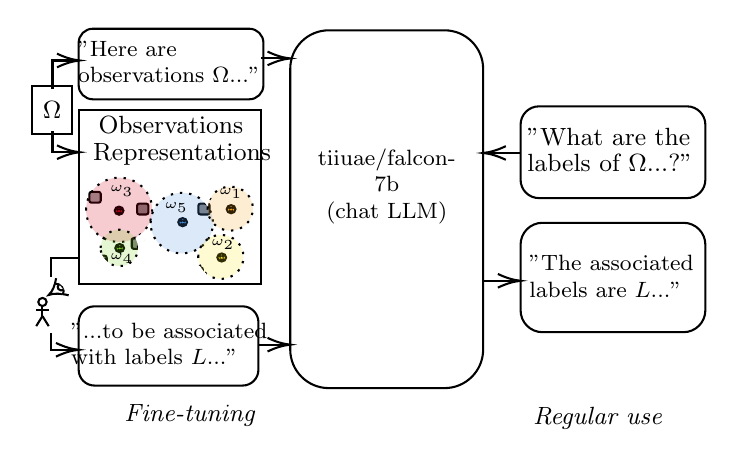
\begin{tikzpicture}[x=0.75pt,y=0.75pt,yscale=-1,xscale=1]
%uncomment if require: \path (0,2218); %set diagram left start at 0, and has height of 2218

%Rounded Rect [id:dp3065899737796194] 
\draw   (164.06,581.82) .. controls (164.06,578.07) and (167.1,575.02) .. (170.86,575.02) -- (246.28,575.02) .. controls (250.03,575.02) and (253.08,578.07) .. (253.08,581.82) -- (253.08,602.22) .. controls (253.08,605.98) and (250.03,609.02) .. (246.28,609.02) -- (170.86,609.02) .. controls (167.1,609.02) and (164.06,605.98) .. (164.06,602.22) -- cycle ;
%Rounded Rect [id:dp21207081175468856] 
\draw   (266,594.37) .. controls (266,584.1) and (274.32,575.78) .. (284.59,575.78) -- (340.35,575.78) .. controls (350.62,575.78) and (358.94,584.1) .. (358.94,594.37) -- (358.94,729.59) .. controls (358.94,739.85) and (350.62,748.17) .. (340.35,748.17) -- (284.59,748.17) .. controls (274.32,748.17) and (266,739.85) .. (266,729.59) -- cycle ;
%Rounded Rect [id:dp19241956316681819] 
\draw  [fill={rgb, 255:red, 128; green, 128; blue, 128 }  ,fill opacity=1 ] (189.63,676.91) .. controls (189.63,676.33) and (190.1,675.86) .. (190.68,675.86) -- (194.07,675.86) .. controls (194.65,675.86) and (195.11,676.33) .. (195.11,676.91) -- (195.11,680.05) .. controls (195.11,680.63) and (194.65,681.1) .. (194.07,681.1) -- (190.68,681.1) .. controls (190.1,681.1) and (189.63,680.63) .. (189.63,680.05) -- cycle ;
%Rounded Rect [id:dp17029144454879885] 
\draw  [fill={rgb, 255:red, 128; green, 128; blue, 128 }  ,fill opacity=1 ] (218.45,691.09) .. controls (218.45,690.52) and (218.92,690.05) .. (219.5,690.05) -- (222.89,690.05) .. controls (223.47,690.05) and (223.94,690.52) .. (223.94,691.09) -- (223.94,694.23) .. controls (223.94,694.81) and (223.47,695.28) .. (222.89,695.28) -- (219.5,695.28) .. controls (218.92,695.28) and (218.45,694.81) .. (218.45,694.23) -- cycle ;
%Rounded Rect [id:dp19487907515171776] 
\draw  [fill={rgb, 255:red, 128; green, 128; blue, 128 }  ,fill opacity=1 ] (172.13,685.42) .. controls (172.13,684.84) and (172.6,684.37) .. (173.17,684.37) -- (176.57,684.37) .. controls (177.14,684.37) and (177.61,684.84) .. (177.61,685.42) -- (177.61,688.56) .. controls (177.61,689.14) and (177.14,689.61) .. (176.57,689.61) -- (173.17,689.61) .. controls (172.6,689.61) and (172.13,689.14) .. (172.13,688.56) -- cycle ;
%Shape: Smiley Face [id:dp41921632791206664] 
\draw  [fill={rgb, 255:red, 208; green, 2; blue, 27 }  ,fill opacity=1 ] (181.43,662.68) .. controls (181.43,661.6) and (182.37,660.73) .. (183.53,660.73) .. controls (184.7,660.73) and (185.64,661.6) .. (185.64,662.68) .. controls (185.64,663.75) and (184.7,664.63) .. (183.53,664.63) .. controls (182.37,664.63) and (181.43,663.75) .. (181.43,662.68) -- cycle ; \draw  [fill={rgb, 255:red, 208; green, 2; blue, 27 }  ,fill opacity=1 ] (182.61,662.02) .. controls (182.61,661.91) and (182.7,661.82) .. (182.82,661.82) .. controls (182.93,661.82) and (183.03,661.91) .. (183.03,662.02) .. controls (183.03,662.12) and (182.93,662.21) .. (182.82,662.21) .. controls (182.7,662.21) and (182.61,662.12) .. (182.61,662.02) -- cycle ; \draw  [fill={rgb, 255:red, 208; green, 2; blue, 27 }  ,fill opacity=1 ] (184.04,662.02) .. controls (184.04,661.91) and (184.14,661.82) .. (184.25,661.82) .. controls (184.37,661.82) and (184.46,661.91) .. (184.46,662.02) .. controls (184.46,662.12) and (184.37,662.21) .. (184.25,662.21) .. controls (184.14,662.21) and (184.04,662.12) .. (184.04,662.02) -- cycle ; \draw   (182.48,663.46) .. controls (183.18,663.98) and (183.89,663.98) .. (184.59,663.46) ;
%Shape: Smiley Face [id:dp39460900412711575] 
\draw  [fill={rgb, 255:red, 126; green, 211; blue, 33 }  ,fill opacity=1 ] (181.72,680.69) .. controls (181.72,679.62) and (182.66,678.75) .. (183.83,678.75) .. controls (184.99,678.75) and (185.94,679.62) .. (185.94,680.69) .. controls (185.94,681.77) and (184.99,682.64) .. (183.83,682.64) .. controls (182.66,682.64) and (181.72,681.77) .. (181.72,680.69) -- cycle ; \draw  [fill={rgb, 255:red, 126; green, 211; blue, 33 }  ,fill opacity=1 ] (182.9,680.03) .. controls (182.9,679.92) and (182.99,679.84) .. (183.11,679.84) .. controls (183.23,679.84) and (183.32,679.92) .. (183.32,680.03) .. controls (183.32,680.14) and (183.23,680.23) .. (183.11,680.23) .. controls (182.99,680.23) and (182.9,680.14) .. (182.9,680.03) -- cycle ; \draw  [fill={rgb, 255:red, 126; green, 211; blue, 33 }  ,fill opacity=1 ] (184.33,680.03) .. controls (184.33,679.92) and (184.43,679.84) .. (184.54,679.84) .. controls (184.66,679.84) and (184.75,679.92) .. (184.75,680.03) .. controls (184.75,680.14) and (184.66,680.23) .. (184.54,680.23) .. controls (184.43,680.23) and (184.33,680.14) .. (184.33,680.03) -- cycle ; \draw   (182.77,681.47) .. controls (183.47,681.99) and (184.18,681.99) .. (184.88,681.47) ;
%Rounded Rect [id:dp7113850974884091] 
\draw  [fill={rgb, 255:red, 128; green, 128; blue, 128 }  ,fill opacity=1 ] (192.2,660.33) .. controls (192.2,659.75) and (192.67,659.28) .. (193.24,659.28) -- (196.63,659.28) .. controls (197.21,659.28) and (197.68,659.75) .. (197.68,660.33) -- (197.68,663.47) .. controls (197.68,664.04) and (197.21,664.51) .. (196.63,664.51) -- (193.24,664.51) .. controls (192.67,664.51) and (192.2,664.04) .. (192.2,663.47) -- cycle ;
%Rounded Rect [id:dp7077104329157917] 
\draw  [fill={rgb, 255:red, 128; green, 128; blue, 128 }  ,fill opacity=1 ] (221.72,660.33) .. controls (221.72,659.75) and (222.19,659.28) .. (222.77,659.28) -- (226.16,659.28) .. controls (226.73,659.28) and (227.2,659.75) .. (227.2,660.33) -- (227.2,663.47) .. controls (227.2,664.04) and (226.73,664.51) .. (226.16,664.51) -- (222.77,664.51) .. controls (222.19,664.51) and (221.72,664.04) .. (221.72,663.47) -- cycle ;
%Rounded Rect [id:dp3685137468405393] 
\draw  [fill={rgb, 255:red, 155; green, 155; blue, 155 }  ,fill opacity=1 ] (169.21,654.65) .. controls (169.21,654.07) and (169.68,653.6) .. (170.26,653.6) -- (173.65,653.6) .. controls (174.23,653.6) and (174.7,654.07) .. (174.7,654.65) -- (174.7,657.79) .. controls (174.7,658.37) and (174.23,658.84) .. (173.65,658.84) -- (170.26,658.84) .. controls (169.68,658.84) and (169.21,658.37) .. (169.21,657.79) -- cycle ;
%Shape: Smiley Face [id:dp2560757002578422] 
\draw  [fill={rgb, 255:red, 245; green, 166; blue, 35 }  ,fill opacity=1 ] (235.39,661.97) .. controls (235.39,660.89) and (236.34,660.02) .. (237.5,660.02) .. controls (238.67,660.02) and (239.61,660.89) .. (239.61,661.97) .. controls (239.61,663.04) and (238.67,663.92) .. (237.5,663.92) .. controls (236.34,663.92) and (235.39,663.04) .. (235.39,661.97) -- cycle ; \draw  [fill={rgb, 255:red, 245; green, 166; blue, 35 }  ,fill opacity=1 ] (236.57,661.31) .. controls (236.57,661.2) and (236.67,661.11) .. (236.78,661.11) .. controls (236.9,661.11) and (236.99,661.2) .. (236.99,661.31) .. controls (236.99,661.41) and (236.9,661.5) .. (236.78,661.5) .. controls (236.67,661.5) and (236.57,661.41) .. (236.57,661.31) -- cycle ; \draw  [fill={rgb, 255:red, 245; green, 166; blue, 35 }  ,fill opacity=1 ] (238.01,661.31) .. controls (238.01,661.2) and (238.1,661.11) .. (238.22,661.11) .. controls (238.33,661.11) and (238.43,661.2) .. (238.43,661.31) .. controls (238.43,661.41) and (238.33,661.5) .. (238.22,661.5) .. controls (238.1,661.5) and (238.01,661.41) .. (238.01,661.31) -- cycle ; \draw   (236.45,662.75) .. controls (237.15,663.27) and (237.85,663.27) .. (238.55,662.75) ;
%Shape: Smiley Face [id:dp7266505536918924] 
\draw  [fill={rgb, 255:red, 248; green, 231; blue, 28 }  ,fill opacity=1 ] (230.87,685.23) .. controls (230.87,684.16) and (231.81,683.29) .. (232.98,683.29) .. controls (234.14,683.29) and (235.09,684.16) .. (235.09,685.23) .. controls (235.09,686.31) and (234.14,687.18) .. (232.98,687.18) .. controls (231.81,687.18) and (230.87,686.31) .. (230.87,685.23) -- cycle ; \draw  [fill={rgb, 255:red, 248; green, 231; blue, 28 }  ,fill opacity=1 ] (232.05,684.57) .. controls (232.05,684.46) and (232.15,684.38) .. (232.26,684.38) .. controls (232.38,684.38) and (232.47,684.46) .. (232.47,684.57) .. controls (232.47,684.68) and (232.38,684.77) .. (232.26,684.77) .. controls (232.15,684.77) and (232.05,684.68) .. (232.05,684.57) -- cycle ; \draw  [fill={rgb, 255:red, 248; green, 231; blue, 28 }  ,fill opacity=1 ] (233.49,684.57) .. controls (233.49,684.46) and (233.58,684.38) .. (233.7,684.38) .. controls (233.81,684.38) and (233.91,684.46) .. (233.91,684.57) .. controls (233.91,684.68) and (233.81,684.77) .. (233.7,684.77) .. controls (233.58,684.77) and (233.49,684.68) .. (233.49,684.57) -- cycle ; \draw   (231.92,686.01) .. controls (232.63,686.53) and (233.33,686.53) .. (234.03,686.01) ;
%Shape: Smiley Face [id:dp11775480475393052] 
\draw  [fill={rgb, 255:red, 74; green, 144; blue, 226 }  ,fill opacity=1 ] (212.05,668.21) .. controls (212.05,667.13) and (213,666.26) .. (214.16,666.26) .. controls (215.33,666.26) and (216.27,667.13) .. (216.27,668.21) .. controls (216.27,669.29) and (215.33,670.16) .. (214.16,670.16) .. controls (213,670.16) and (212.05,669.29) .. (212.05,668.21) -- cycle ; \draw  [fill={rgb, 255:red, 74; green, 144; blue, 226 }  ,fill opacity=1 ] (213.24,667.55) .. controls (213.24,667.44) and (213.33,667.35) .. (213.45,667.35) .. controls (213.56,667.35) and (213.66,667.44) .. (213.66,667.55) .. controls (213.66,667.66) and (213.56,667.74) .. (213.45,667.74) .. controls (213.33,667.74) and (213.24,667.66) .. (213.24,667.55) -- cycle ; \draw  [fill={rgb, 255:red, 74; green, 144; blue, 226 }  ,fill opacity=1 ] (214.67,667.55) .. controls (214.67,667.44) and (214.76,667.35) .. (214.88,667.35) .. controls (215,667.35) and (215.09,667.44) .. (215.09,667.55) .. controls (215.09,667.66) and (215,667.74) .. (214.88,667.74) .. controls (214.76,667.74) and (214.67,667.66) .. (214.67,667.55) -- cycle ; \draw   (213.11,668.99) .. controls (213.81,669.51) and (214.52,669.51) .. (215.22,668.99) ;
%Shape: Ellipse [id:dp39865204793515163] 
\draw  [fill={rgb, 255:red, 208; green, 2; blue, 27 }  ,fill opacity=0.2 ][dash pattern={on 0.84pt off 2.51pt}] (167.64,662.27) .. controls (167.64,653.72) and (174.77,646.78) .. (183.56,646.78) .. controls (192.36,646.78) and (199.49,653.72) .. (199.49,662.27) .. controls (199.49,670.83) and (192.36,677.76) .. (183.56,677.76) .. controls (174.77,677.76) and (167.64,670.83) .. (167.64,662.27) -- cycle ;
%Shape: Ellipse [id:dp33951964171475946] 
\draw  [fill={rgb, 255:red, 74; green, 144; blue, 226 }  ,fill opacity=0.2 ][dash pattern={on 0.84pt off 2.51pt}] (198.75,668.66) .. controls (198.75,660.6) and (205.46,654.07) .. (213.75,654.07) .. controls (222.03,654.07) and (228.75,660.6) .. (228.75,668.66) .. controls (228.75,676.72) and (222.03,683.25) .. (213.75,683.25) .. controls (205.46,683.25) and (198.75,676.72) .. (198.75,668.66) -- cycle ;
%Shape: Ellipse [id:dp5512168099964949] 
\draw  [fill={rgb, 255:red, 245; green, 166; blue, 35 }  ,fill opacity=0.2 ][dash pattern={on 0.84pt off 2.51pt}] (226.18,661.7) .. controls (226.18,655.85) and (231.07,651.09) .. (237.09,651.09) .. controls (243.12,651.09) and (248,655.85) .. (248,661.7) .. controls (248,667.56) and (243.12,672.32) .. (237.09,672.32) .. controls (231.07,672.32) and (226.18,667.56) .. (226.18,661.7) -- cycle ;
%Shape: Ellipse [id:dp7271962621592551] 
\draw  [fill={rgb, 255:red, 248; green, 231; blue, 28 }  ,fill opacity=0.2 ][dash pattern={on 0.84pt off 2.51pt}] (221.66,684.97) .. controls (221.66,679.11) and (226.54,674.36) .. (232.57,674.36) .. controls (238.59,674.36) and (243.48,679.11) .. (243.48,684.97) .. controls (243.48,690.83) and (238.59,695.58) .. (232.57,695.58) .. controls (226.54,695.58) and (221.66,690.83) .. (221.66,684.97) -- cycle ;
%Shape: Ellipse [id:dp2818847294483997] 
\draw  [fill={rgb, 255:red, 126; green, 211; blue, 33 }  ,fill opacity=0.2 ][dash pattern={on 0.84pt off 2.51pt}] (174.65,680.62) .. controls (174.65,675.77) and (178.69,671.84) .. (183.68,671.84) .. controls (188.67,671.84) and (192.71,675.77) .. (192.71,680.62) .. controls (192.71,685.47) and (188.67,689.4) .. (183.68,689.4) .. controls (178.69,689.4) and (174.65,685.47) .. (174.65,680.62) -- cycle ;
%Shape: Polygon [id:ds47995740588172153] 
\draw  [color={rgb, 255:red, 255; green, 255; blue, 255 }  ,draw opacity=1 ][fill={rgb, 255:red, 255; green, 255; blue, 255 }  ,fill opacity=1 ] (171.77,690.16) -- (171.53,683.9) -- (174.64,683.83) -- (175.86,685.93) -- (177.36,687.49) -- (179.34,688.89) -- (179.3,691.09) -- cycle ;
%Shape: Polygon [id:ds5983584727400302] 
\draw  [color={rgb, 255:red, 255; green, 255; blue, 255 }  ,draw opacity=1 ][fill={rgb, 255:red, 255; green, 255; blue, 255 }  ,fill opacity=1 ] (195.67,678.82) -- (195.39,682.56) -- (192.96,682.82) -- (193.28,680.46) -- (193.12,679.08) -- (192.8,677.96) -- (191.99,675.97) -- (193.04,675.3) -- (194.82,674.06) -- cycle ;
%Shape: Polygon [id:ds5117837642106575] 
\draw  [color={rgb, 255:red, 255; green, 255; blue, 255 }  ,draw opacity=1 ][fill={rgb, 255:red, 255; green, 255; blue, 255 }  ,fill opacity=1 ] (166.76,651.77) -- (167.12,650.13) -- (167.77,648.67) -- (169.68,648.85) -- (168.78,649.94) -- (167.73,652) -- (167.24,653.53) -- cycle ;
%Shape: Polygon [id:ds3218436577846133] 
\draw  [color={rgb, 255:red, 255; green, 255; blue, 255 }  ,draw opacity=1 ][fill={rgb, 255:red, 255; green, 255; blue, 255 }  ,fill opacity=1 ] (224.32,696) -- (217.87,695.93) -- (217.51,689.9) -- (222.23,689.81) -- (222.98,690.95) -- (223.91,692.22) -- (225,693.23) -- cycle ;
%Shape: Polygon [id:ds17720973316669864] 
\draw  [color={rgb, 255:red, 255; green, 255; blue, 255 }  ,draw opacity=1 ][fill={rgb, 255:red, 255; green, 255; blue, 255 }  ,fill opacity=1 ] (225.98,659.5) -- (225.49,658.87) -- (224.96,658.23) -- (224.23,657.71) -- (223.75,657.07) -- (227.16,656.25) -- (226.42,657.29) -- (226.26,658.15) -- (226.22,658.75) -- cycle ;
%Shape: Rectangle [id:dp6636168765165942] 
\draw   (164.39,614) -- (252.06,614) -- (252.06,698) -- (164.39,698) -- cycle ;
%Rounded Rect [id:dp024205864664161858] 
\draw   (164.06,716.4) .. controls (164.06,712.19) and (167.48,708.77) .. (171.69,708.77) -- (243.04,708.77) .. controls (247.25,708.77) and (250.67,712.19) .. (250.67,716.4) -- (250.67,739.31) .. controls (250.67,743.53) and (247.25,746.94) .. (243.04,746.94) -- (171.69,746.94) .. controls (167.48,746.94) and (164.06,743.53) .. (164.06,739.31) -- cycle ;
%Straight Lines [id:da6746655718418797] 
\draw    (151.47,603.92) -- (151.47,590.32) -- (162.57,590.32) ;
\draw [shift={(164.57,590.32)}, rotate = 180] [color={rgb, 255:red, 0; green, 0; blue, 0 }  ][line width=0.75]    (10.93,-3.29) .. controls (6.95,-1.4) and (3.31,-0.3) .. (0,0) .. controls (3.31,0.3) and (6.95,1.4) .. (10.93,3.29)   ;
%Straight Lines [id:da8479196030811313] 
\draw    (164.06,685.37) -- (150.83,685.37) -- (150.83,729.7) -- (162.06,729.7) ;
\draw [shift={(164.06,729.7)}, rotate = 180] [color={rgb, 255:red, 0; green, 0; blue, 0 }  ][line width=0.75]    (10.93,-3.29) .. controls (6.95,-1.4) and (3.31,-0.3) .. (0,0) .. controls (3.31,0.3) and (6.95,1.4) .. (10.93,3.29)   ;
%Straight Lines [id:da47773919231179085] 
\draw    (151.47,624.32) -- (151.47,634.52) -- (162.57,634.52) ;
\draw [shift={(164.57,634.52)}, rotate = 180] [color={rgb, 255:red, 0; green, 0; blue, 0 }  ][line width=0.75]    (10.93,-3.29) .. controls (6.95,-1.4) and (3.31,-0.3) .. (0,0) .. controls (3.31,0.3) and (6.95,1.4) .. (10.93,3.29)   ;
%Straight Lines [id:da6453412801076328] 
\draw    (252.13,589.33) -- (264,589.33) ;
\draw [shift={(266,589.33)}, rotate = 180] [color={rgb, 255:red, 0; green, 0; blue, 0 }  ][line width=0.75]    (10.93,-3.29) .. controls (6.95,-1.4) and (3.31,-0.3) .. (0,0) .. controls (3.31,0.3) and (6.95,1.4) .. (10.93,3.29)   ;
%Shape: Rectangle [id:dp3955964166837225] 
\draw  [color={rgb, 255:red, 255; green, 255; blue, 255 }  ,draw opacity=1 ][fill={rgb, 255:red, 255; green, 255; blue, 255 }  ,fill opacity=1 ] (140,695.22) -- (160.45,695.22) -- (160.45,721.08) -- (140,721.08) -- cycle ;
%Shape: Ellipse [id:dp6608885205864825] 
\draw  [fill={rgb, 255:red, 255; green, 255; blue, 255 }  ,fill opacity=1 ] (144.61,706.67) .. controls (144.61,705.6) and (145.51,704.73) .. (146.62,704.73) .. controls (147.73,704.73) and (148.63,705.6) .. (148.63,706.67) .. controls (148.63,707.75) and (147.73,708.61) .. (146.62,708.61) .. controls (145.51,708.61) and (144.61,707.75) .. (144.61,706.67) -- cycle ;
%Straight Lines [id:da5798058819230947] 
\draw [fill={rgb, 255:red, 255; green, 255; blue, 255 }  ,fill opacity=1 ]   (146.62,708.61) -- (146.62,713.46) ;
%Straight Lines [id:da9388770820150178] 
\draw [fill={rgb, 255:red, 255; green, 255; blue, 255 }  ,fill opacity=1 ]   (146.62,713.46) -- (143.61,718.31) ;
%Straight Lines [id:da4442933898118544] 
\draw [fill={rgb, 255:red, 255; green, 255; blue, 255 }  ,fill opacity=1 ]   (146.62,713.46) -- (149.63,718.31) ;
%Straight Lines [id:da43183325949182816] 
\draw [fill={rgb, 255:red, 255; green, 255; blue, 255 }  ,fill opacity=1 ]   (149.63,710.55) -- (143.61,710.55) ;

\draw  [fill={rgb, 255:red, 255; green, 255; blue, 255 }  ,fill opacity=1 ] (159.25,703.45) .. controls (155.37,702.48) and (152.16,702.42) .. (149.63,703.29) .. controls (151.49,701.51) and (152.68,698.82) .. (153.18,695.22) ;
%Shape: Arc [id:dp8028068753225497] 
\draw  [draw opacity=0][fill={rgb, 255:red, 255; green, 255; blue, 255 }  ,fill opacity=1 ] (152.7,697.84) .. controls (153.8,697.68) and (155.17,698.33) .. (156.06,699.53) .. controls (156.94,700.73) and (157.08,702.1) .. (156.51,702.96) -- (153.97,700.79) -- cycle ; \draw   (152.7,697.84) .. controls (153.8,697.68) and (155.17,698.33) .. (156.06,699.53) .. controls (156.94,700.73) and (157.08,702.1) .. (156.51,702.96) ;  
%Shape: Arc [id:dp427165213423107] 
\draw  [draw opacity=0][fill={rgb, 255:red, 255; green, 255; blue, 255 }  ,fill opacity=1 ] (154.55,698.31) .. controls (153.9,698.83) and (153.77,699.72) .. (154.27,700.4) .. controls (154.82,701.14) and (155.92,701.35) .. (156.73,700.87) .. controls (156.73,700.87) and (156.73,700.86) .. (156.74,700.86) -- (155.74,699.52) -- cycle ; \draw   (154.55,698.31) .. controls (153.9,698.83) and (153.77,699.72) .. (154.27,700.4) .. controls (154.82,701.14) and (155.92,701.35) .. (156.73,700.87) .. controls (156.73,700.87) and (156.73,700.86) .. (156.74,700.86) ;  



%Straight Lines [id:da2725108503030351] 
\draw    (250.67,727.24) -- (264,727.24) ;
\draw [shift={(266,727.24)}, rotate = 180] [color={rgb, 255:red, 0; green, 0; blue, 0 }  ][line width=0.75]    (10.93,-3.29) .. controls (6.95,-1.4) and (3.31,-0.3) .. (0,0) .. controls (3.31,0.3) and (6.95,1.4) .. (10.93,3.29)   ;
%Rounded Rect [id:dp7178386003297756] 
\draw   (376.98,621.26) .. controls (376.98,616.38) and (380.94,612.42) .. (385.82,612.42) -- (457.16,612.42) .. controls (462.04,612.42) and (466,616.38) .. (466,621.26) -- (466,647.78) .. controls (466,652.66) and (462.04,656.62) .. (457.16,656.62) -- (385.82,656.62) .. controls (380.94,656.62) and (376.98,652.66) .. (376.98,647.78) -- cycle ;
%Rounded Rect [id:dp8093118952391012] 
\draw   (376.98,679.06) .. controls (376.98,673.24) and (381.7,668.52) .. (387.52,668.52) -- (455.46,668.52) .. controls (461.28,668.52) and (466,673.24) .. (466,679.06) -- (466,710.68) .. controls (466,716.5) and (461.28,721.22) .. (455.46,721.22) -- (387.52,721.22) .. controls (381.7,721.22) and (376.98,716.5) .. (376.98,710.68) -- cycle ;
%Straight Lines [id:da6033397776174121] 
\draw    (358.94,696.46) -- (374.98,696.46) ;
\draw [shift={(376.98,696.46)}, rotate = 180] [color={rgb, 255:red, 0; green, 0; blue, 0 }  ][line width=0.75]    (10.93,-3.29) .. controls (6.95,-1.4) and (3.31,-0.3) .. (0,0) .. controls (3.31,0.3) and (6.95,1.4) .. (10.93,3.29)   ;
%Straight Lines [id:da23835330101425622] 
\draw    (376.98,634.89) -- (360.94,634.89) ;
\draw [shift={(358.94,634.89)}, rotate = 360] [color={rgb, 255:red, 0; green, 0; blue, 0 }  ][line width=0.75]    (10.93,-3.29) .. controls (6.95,-1.4) and (3.31,-0.3) .. (0,0) .. controls (3.31,0.3) and (6.95,1.4) .. (10.93,3.29)   ;


% Text Node
\draw (420.8,694.27) node  [font=\footnotesize] [align=left] {"The associated\\labels are $\displaystyle L$..."};
% Text Node
\draw (414.5,762.5) node  [font=\small] [align=left] {\textit{Regular use}};
% Text Node
\draw (420.19,633.5) node  [font=\footnotesize] [align=left] {{\small "What are the}\\{\small labels of $\displaystyle \Omega $...?"}};
% Text Node
\draw    (141.77,602.71) -- (160.77,602.71) -- (160.77,625.71) -- (141.77,625.71) -- cycle  ;
\draw (151.27,614.21) node  [font=\small] [align=left] {{\small $\displaystyle \Omega $}};
% Text Node
\draw (211.17,661.31) node  [font=\tiny] [align=left] {$\displaystyle \omega _{5}$};
% Text Node
\draw (184.92,685.57) node  [font=\tiny] [align=left] {$\displaystyle \omega _{4}$};
% Text Node
\draw (184.92,653.23) node  [font=\tiny] [align=left] {$\displaystyle \omega _{3}$};
% Text Node
\draw (233.54,678.83) node  [font=\tiny] [align=left] {$\displaystyle \omega _{2}$};
% Text Node
\draw (237.43,654.58) node  [font=\tiny] [align=left] {$\displaystyle \omega _{1}$};
% Text Node
\draw (208.5,629) node  [font=\footnotesize] [align=left] {\begin{minipage}[lt]{56.2pt}\setlength\topsep{0pt}
\begin{center}
{\small Observations}\\{\small Representations}
\end{center}

\end{minipage}};
% Text Node
\draw (218.01,761.37) node  [font=\small] [align=left] {\textit{Fine-tuning}};
% Text Node
\draw (207.69,727) node  [font=\footnotesize] [align=left] {{\footnotesize "...to be associated}\\{\footnotesize with labels $\displaystyle L$..."}};
% Text Node
\draw (312.5,651) node  [font=\footnotesize] [align=left] {\begin{minipage}[lt]{58.07pt}\setlength\topsep{0pt}
\begin{center}
tiiuae/falcon-7b\\(chat LLM)
\end{center}

\end{minipage}};
% Text Node
\draw (207.75,591) node  [font=\footnotesize] [align=left] {{\footnotesize "Here are}\\{\footnotesize observations $\displaystyle \Omega $..."}};


\end{tikzpicture}